\documentclass[11pt]{article}
\usepackage[T1]{fontenc}
\usepackage[margin=0.82in]{geometry}
\usepackage{amsmath,amssymb}
\usepackage{booktabs,tabularx}
\usepackage{graphicx}
\usepackage[hidelinks]{hyperref}
\usepackage{microtype}

\newcommand{\R}{\mathbb R}
\newcommand{\N}{\mathbb N}
\newcommand{\Pos}{\operatorname{Pos}}

\title{Variable-coefficient positivity generators on $\R^n$}
\author{Literature-already-answered note for arXiv:2308.10455}
\date{11 August 2026}

\begin{document}
\maketitle

\paragraph{Status.}
\textbf{Open Problem 6.1 is completely answered by di Dio--Schm\"udgen,
arXiv:2407.15654, Theorem~5.12.}
The later theorem treats exactly the same degree-preserving canonical
differential operators and gives a necessary-and-sufficient pointwise
L\'evy--Khintchine description.  This packet records that later-literature
resolution; it does not claim a new theorem.

\section*{The source problem}
Let $\Pos(\R^n)$ denote the cone of real polynomials nonnegative on
$\R^n$.  The source observes that a linear operator on
$\R[x_1,\ldots,x_n]$ is degree preserving precisely when it has the
canonical representation
\[
 A=\sum_{\alpha\in\N_0^n}q_\alpha(x)\,\partial^\alpha,
 \qquad \deg q_\alpha\le |\alpha|.
\]
This condition makes $e^{tA}$ well defined on every finite-degree
polynomial subspace.  Open Problem~6.1 on source PDF page~22 asks for a
description of all such $A$, without the constant-coefficient restriction,
for which
\[
 e^{tA}\Pos(\R^n)\subseteq\Pos(\R^n)\qquad(t\ge0).
\]

\begin{center}

\includegraphics[width=0.64\textwidth]{evidence/source_open_problem_crop.png}

{\footnotesize Source evidence: arXiv:2308.10455, PDF page 22 (unaltered crop).}
\end{center}

\clearpage
\section*{The exact later theorem}
Theorem~5.12 of arXiv:2407.15654 (PDF page~25) writes the same operator as
\[
 A=\sum_{\alpha\in\N_0^n}\frac{a_\alpha(x)}{\alpha!}\partial^\alpha,
 \qquad a_\alpha\in\R[x_1,\ldots,x_n]_{\le |\alpha|}.
\]
It proves that $e^{tA}$ preserves $\Pos(\R^n)$ for every $t\ge0$ if and
only if, for every $y\in\R^n$, there are a positive-semidefinite symmetric
matrix $\Sigma(y)=(\sigma_{ij}(y))$, a drift vector
$b(y)=(b_1(y),\ldots,b_n(y))^T$, and a measure $\nu_y$ on $\R^n$ such that
\[
 \int_{\|z\|_2\ge1}|z_i|\,d\nu_y(z)<\infty,
 \qquad
 \int_{\R^n}|z^\alpha|\,d\nu_y(z)<\infty\quad(|\alpha|\ge2),
\]
and the coefficient values obey
\begin{align*}
 a_{e_i}(y)
  &=b_i(y)+\int_{\|z\|_2\ge1}z_i\,d\nu_y(z),\\
 a_{e_i+e_j}(y)
  &=\sigma_{ij}(y)+\int_{\R^n}z^{e_i+e_j}\,d\nu_y(z),\\
 a_\alpha(y)
  &=\int_{\R^n}z^\alpha\,d\nu_y(z)\qquad(|\alpha|\ge3).
\end{align*}
Here $a_0$ is an arbitrary real constant, as forced already by
$\deg a_0\le0$.  Thus the zeroth-order scaling, drift, Gaussian part, and
jump moments give the requested complete description.

\section*{Why this is the same question}
Set $a_\alpha=\alpha!q_\alpha$.  This is a bijective change of
normalization and preserves the bound $\deg a_\alpha\le|\alpha|$.  Both
papers use the same cone of globally nonnegative polynomials, the same
semigroup condition for every $t\ge0$, and arbitrary polynomial (not merely
constant) coefficients.

\begin{center}
\small
\begin{tabularx}{\textwidth}{@{}p{0.25\textwidth}XX@{}}
\toprule
Feature & Open Problem 6.1 & Theorem 5.12 \\
\midrule
Operator class
 & $\sum q_\alpha\partial^\alpha$, $\deg q_\alpha\le|\alpha|$
 & $\sum(a_\alpha/\alpha!)\partial^\alpha$, same bound \\
Positivity domain
 & all of $\R^n$
 & $K=\R^n$ \\
Requested property
 & $e^{tA}$ positive for all $t\ge0$
 & condition (i), verbatim \\
Requested output
 & description of every generator
 & iff L\'evy--Khintchine data at every $y$ \\
\bottomrule
\end{tabularx}
\end{center}

\clearpage
\section*{Proof intuition}
For each point $y$, freeze the polynomial coefficients:
\[
 A_y=\sum_\alpha\frac{a_\alpha(y)}{\alpha!}\partial^\alpha.
\]
The key result behind Theorem~5.12 is the equivalence
\[
 A\text{ generates a positivity-preserving semigroup}
 \quad\Longleftrightarrow\quad
 A_y\text{ does so for every }y\in\R^n.
\]
The forward direction uses translation invariance of each constant-
coefficient $A_y$, together with the first-order expansion of $e^{tA}$ and
a product-limit argument.  The reverse direction constructs positive
approximants from the frozen semigroups and again takes a closed product
limit.  The already-solved constant-coefficient generator theorem then
applies pointwise.  Its L\'evy--Khintchine formula is exactly the matrix,
drift, and measure condition displayed above.  This explains both why the
answer is pointwise in $y$ and why no compatibility conditions beyond the
given polynomial coefficient functions are missing.

\begin{center}
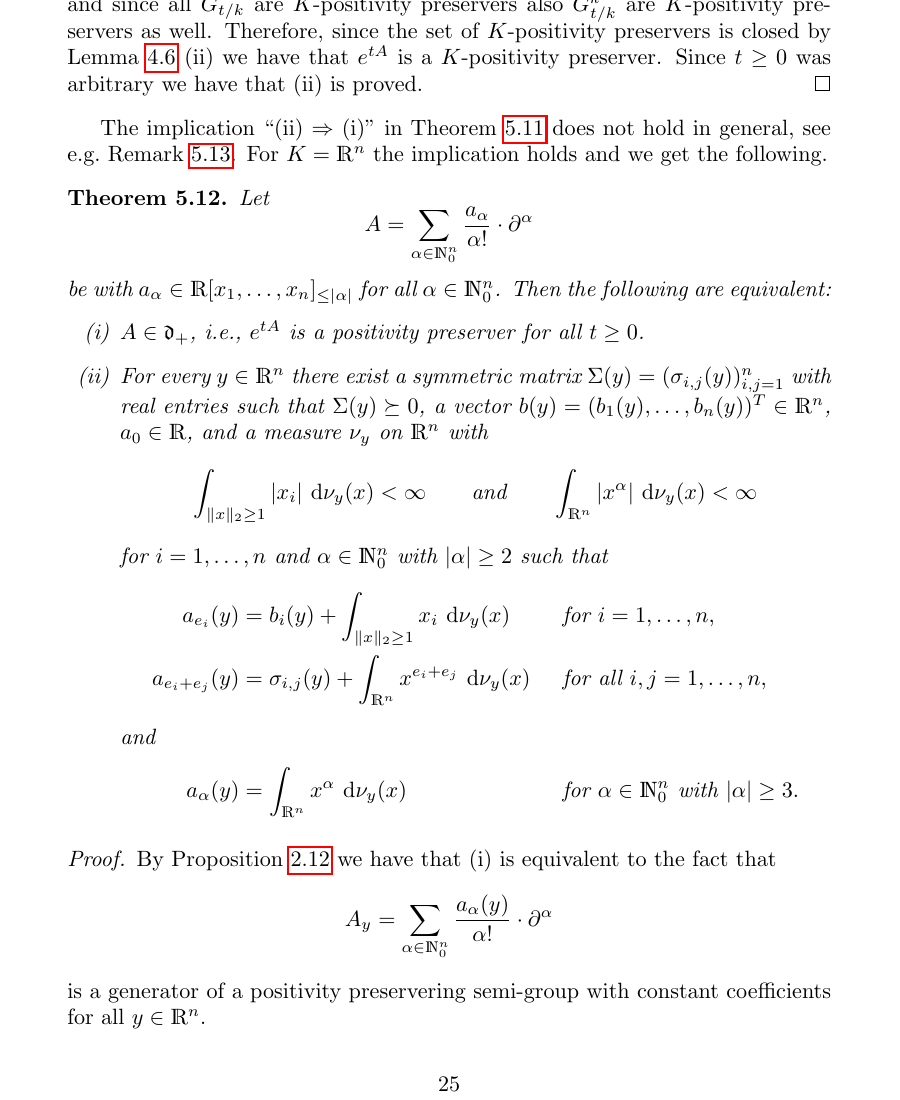
\includegraphics[width=0.68\textwidth]{evidence/support_theorem_5_12_crop.png}

{\footnotesize Supporting evidence: arXiv:2407.15654, Theorem 5.12 on PDF
page 25 (unaltered crop).}
\end{center}

\paragraph{Human review.}
Compare Open Problem~6.1 on source PDF page~22 with Theorem~5.12 on
supporting PDF page~25.  In particular, verify the harmless normalization
$a_\alpha=\alpha!q_\alpha$ and the shared degree bound.

\begin{thebibliography}{9}
\raggedright
\bibitem{source}
P. J. di Dio,
\emph{On Positivity Preservers with constant Coefficients and their
Generators}, arXiv:2308.10455.  See Open Problem~6.1, PDF page~22.

\bibitem{answer}
P. J. di Dio and K. Schm\"udgen,
\emph{$K$-Positivity Preservers and their Generators}, arXiv:2407.15654.
See Theorem~5.12, PDF page~25.
\end{thebibliography}

\end{document}
